\documentclass[12pt, centerh1]{article}
\textwidth=165mm \headheight=0mm \headsep=10mm \topmargin=-10mm
\textheight=230mm %\footskip=1.5cm
\oddsidemargin=0mm
%\documentclass[12pt,letterpaper]{article}
%\usepackage[margin=1in]{geometry}
\RequirePackage[colorlinks,citecolor=blue,urlcolor=blue]{hyperref}
\usepackage{amsmath, amssymb,natbib}
%\usepackage[mathscr]{euscript}
%\usepackage{mathrsfs}
\usepackage{graphicx,bm}
\usepackage{color}
\usepackage{subcaption}
\usepackage{subcaption}
\usepackage[table]{xcolor}
\usepackage{longtable}
\usepackage{amsthm}
\usepackage[mathscr]{euscript}
\usepackage{relsize}
\usepackage{amsmath,tabularx}
\newcolumntype{P}[1]{>{\centering\arraybackslash}p{#1}}
\usepackage{rotating}
\usepackage{eurosym}
\usepackage{colonequals}
\usepackage{bbm}
\usepackage{lscape}
\usepackage{natbib}
\usepackage{blindtext}
\usepackage{titlesec}

%%% make comments using the following setup %%
% type \your name {comment}, 
% e.g. \sophie{i love Lyme disease}
\newcommand{\bruce}[1]{{\textcolor{blue}{$\langle$BC: #1$\rangle$}}}
\newcommand{\sophie}[1]{{\textcolor{purple}{$\langle$SS: #1$\rangle$}}}
\newcommand{\lauren}[1]{{\textcolor{cyan}{$\langle$LF: #1$\rangle$}}}
\newcommand{\geneva}[1]{{\textcolor{red}{$\langle$GL: #1$\rangle$}}}
\newcommand{\thanesh}[1]{{\textcolor{yellow}{$\langle$TR: #1$\rangle$}}}

\title{Topical Acaricides on Rodents as a One Health Intervention Against Lyme Disease: A Epidemiological Modelling Study}

%%% put in alphabetical order
\author{Bruce Chidley$^{1}$ \qquad Lauren Farrell$^{2}$ \qquad\  Geneva Liwag$^{2}$ \qquad\  \\  Thaneswary Rajanderan$^{3}$ \quad\ Sophie Stelmach$^{4}$}

\date{{\small $^1$ Department of Computing, Queen's University, Ontario, Canada.\\[-6pt]
$^2$ Department of Mathematics \& Statistics, York University, Ontario, Canada.\\[-6pt]
$^3$ Faculty of Medicine, Memorial University of Newfoundland, Newfoundland, Canada. \\[-6pt]
$^4$ Department of Mathematics \& Statistics, McMaster University, Ontario, Canada.\\[-6pt]
}
}
\linespread{1.5}
\pdfminorversion=4

\begin{document}



\maketitle
{
\hypersetup{linkcolor = black}
\tableofcontents
}
\newpage

\section{Introduction}
Lyme disease (LD) is a highly emerging vector-borne disease in North America, which is caused by the bacterium \textit{Borrelia} and transmitted via infected bites of black-legged ticks (\textit{Ixodes}) \citep{govcan}. The risk of disease is further propagated and has become an increasing concern in Canada due to the changes in migratory patterns northward of these ticks by climate change.

\subsection{Lyme Disease and Tick-host relationships}
\textbf{\textit{Borrelia}}, such as \textit{B. burgdorferi sensu lato}, is the pathogenic spirochete that causes Lyme disease in humans via infected black-legged tick bites \citep{CDC_2022}. Typically, the progression of disease in humans post-bite can be divided into three categories: early localized disease, early disseminated disease, and late persistent disease \citep{MyHealth_Alberta}. Once an infected tick bite, the patient will develop a circular red rash within one month \citep{borrelia_shapiro}. Once the disease begins to disseminate, the patient may develop multiple rashes, flu-like symptoms and cranial nerve palsies. If left untreated for months, patients can transition to the late persistent stage of the disease, where they can develop arthritis, encephalitis, and polyneuropathy conditions \citep{borrelia_shapiro}. 
%\sophie{I edited to get rid of jargon. our audience (especially policy makers) arent all biology experts nor do they care about the specific medical terminology of what lyme disease does. they know its bad and thats enough lol} \thanesh{sounds good!}

\textbf{Black-legged tick}, also known as \textit{I. scapularis}, is the primary cause of LD in Eastern North America, but is also a vector for many pathogens and can also increase the risk %\sophie{for transmitting? this doesnt make sense. how do they increase the risk of polymicrobial infections} \thanesh{since they carry multiple pathogens, the can infect a single host with various microbes that can be disease-causing.}
of transmission of many polymicrobial infections \citep{paulson2023multiomics}. To understand the infectious nature of the tick, it is vital to explore its interaction with multiple hosts throughout its life cycle. Ticks encounter various hosts at different points during their development and have different feeding rates during each stage (see Figure \ref{fig:lifecycle}) \citep{CDC_2022, radolf2012ticks}. When the eggs hatch, the larvae develop by feeding small mammals and birds. Since the ticks are naive when hatching, they get infected with the \textit{borrelia} bacteria at this feeding stage, as small mammals and birds are carriers of this bacteria.
As the larvae develop into nymphs, they seek new hosts. They can feed on rodents, birds, humans, and other small mammals at this stage. So, infected ticks can feed on humans (terminal hosts) and infect them with \textit{B. burgdorferi sensu lato}, leading to Lyme disease \citep{radolf2012ticks}. 
Small mammals such as dogs and cats are incidental hosts who can also get bitten by infected nymph and potentially carry the ticks into households. Once nymphs develop into adult ticks, they feed, mate and lay eggs on only deer, which are essential for tick breeding and propagation. Infected ticks pose the highest risk to humans during the nymph stages as that is where the ticks first encounter the bacteria and can transmit it to humans or incidental hosts around humans \citep{radolf2012ticks}. 
%\sophie{according to CDC's guide to lyme disease, adult ticks bite humans as well but pose less "risk" because they are more easily visible and can be removed earlier. nymph ticks are more risk for giving humans lyme because they are smaller and harder to see and remove. also cdc doesnt say that nymphs bite humans that much?} \thanesh{yup, you are right. fixed it}

\textbf{Lyme disease in Canada}.
Lyme disease is becoming a growing concern in Canada. A study in eastern and southern Ontario, Canada found \textit{Borrelia} sp in approximately 70 percent of ticks with a relative abundance of 0.01 percent of adult \textit{I. scapularis} carrying endosymbiotic and pathogenic microorganisms in Southeastern Ontario \citep{paulson2023multiomics} \citep{clow2018microbiota}. If infections are to continue at the current rate, Lyme disease poses a large burden on the healthcare system in Canada as the cost of treatment will increase with the number of cases. Hence, it is essential to consider preventative interventions as a means to control and reduce the number of cases in this region. 

\subsection{Intervention}

A study by \citet{dolan2004control} evaluated the efficacy of Fipronil, a rodent-targeted acaricide that is placed in bait boxes that rodents visit. Bait boxes such as the ones used in the study by \citet{dolan2004control} are commercially available, and the authors found that the lowest concentration of Fipronil required to kill tick nymphs was 20 $\mu l$. To maintain a regular rate of visiting rodents, the box baits were placed $\sim$10m apart from each other along a rodent path and re-baited and replenished with Fipronil every four weeks. In total, \citet{dolan2004control} report an 89\% reduction in the number of ticks per mouse and a 53\% decrease in the infection rate of ticks present on mice. After their three-year experiment, only 33\% of adult ticks were infected with Lyme disease in sites with the bait boxes, compared to 47\% on sites without the bait boxes. The other advantage to these bait boxes is that many different tick hosts can visit a box and be treated with the acaricide and that minimal environmental impact has been detected \citep{dolan2004control}. 

There is a potential for using bait boxes with acaricide treatment to prevent Lyme disease at the host level. This paper will evaluate the effect of rodents visiting bait boxes and how the tick populations respond to the intervention.

\subsection{Study Objective}

In this study, an existing mathematical model was investigated to evaluate the efficacy of acaricides as a Lyme disease intervention during the tick larval growth stage in Ontario, Canada. The potential for acaricides as an intervention has not been widely researched yet, and could prove useful as a way to control Lyme disease by killing ticks that feed on rodents. 

\begin{figure}[h]
    \centering
    \includegraphics[scale = 0.15]{figures/Tick life cycle and progression of Lyme disease.png}
    \caption{Diagram of tick life cycle and host bias.}
    \label{fig:lifecycle}
\end{figure}

\section{Methods}

\subsection{Proposed model}
The model proposed by \citet{tosato2021host} describes the tick life cycle and disease transmission between the tick and its host and will serve as our base model. The model features compartments that represent the various stages of the tick life cycle: larval ($L$), nymphal ($N$), and adult ($A$). Here, only the nymphal ticks are classified as uninfected/susceptible ($N_S$) or infected ($N_I$). The total rodent population ($H$) is stratified based on status in disease progression: susceptible ($H_S$), infected ($H_I$), or immune ($H_R$), as shown in Figure \ref{fig:flowchart}.

\begin{figure}[h]
    \centering
    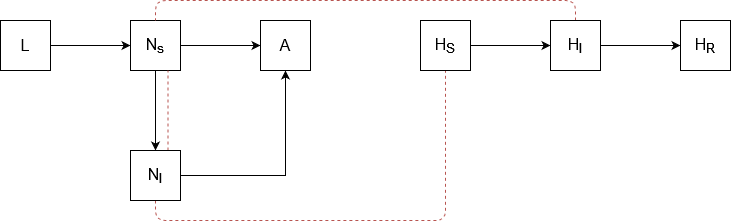
\includegraphics[width=\textwidth]{figures/acaricide_diagram.png}
    \caption{Flow diagram of tick life cycle (including infected nymphal ticks), and disease progression of rodents. Dotted lines indicate interactions that cause disease transmission.}
    \label{fig:flowchart}
\end{figure}

This model considers ticks' birth and death rates, the rates at which they feed on rodents in their respective stages of life, and their slightly varying Lyme disease transmission rates. While ticks feed on their hosts in any life cycle stage, they primarily pose a risk to humans in the nymphal and adult stages. Similarly, ticks will only feed on small rodents during the larval and nymphal stages, at which point these rodents risk acquiring Lyme disease-causing bacteria \citep{borrelia_shapiro}. Thus, tick compartments in the model that deal with disease transmission are only applied to the nymphal stage.

The model considers two main methods of Lyme disease transmission. In the direct or systemic transmission, susceptible larval or nymphal ticks attach to an infected rodent, and become infected with probability $p_{HL}$ or $p_{HN}$ respectively. An infected nymph can also feed onto a susceptible rodent, causing infection with probability $p_{NH}$.

On the other hand, co-feeding or non-systemic transmission occurs between an infected tick and an uninfected tick that feed onto the same rodent in close proximity \citep{voordouw2015co}. Successful tick-tick disease transmission from co-feeding depends on the number of infected nymphs in a given time, and is described by the co-feeding transmission probability $\displaystyle c = 1 - (1-\delta)^{\frac{N_I}{(1-r)H}}$ \citep{tosato2021host,nah2019assessing}. Here, $\delta$ is the probability of co-feeding to a single infected nymph.


The dynamical system from \citet{tosato2021host} is as follows:
\begin{align*}
    \frac{dL(t)}{dt} &= \beta \,A \, e^{-\gamma A} - b_L \,L (1-r) - \mu_L \,L \\
    \frac{dN_S(t)}{dt} &= b_L\,L(1-r)(1-a)(1-c) \, \frac{[H_s + (1- p_{HL})H_I + H_R]}{H} - b_n\,N_S (1-r) \\ 
    \frac{dN_I(t)}{dt} &= b_L \,L(1-r) (1-a) p_{HL} \frac{H_I}{H} + b_L \,L(1-r)(1-a)\,\frac{c \,[H_s + (1- p_{HL})H_I + H_R]}{H} \\
    &- b_N\, N_I (1-r) - \mu_N \,N_I\\
    \frac{dA(t)}{dt} &= b_N \,(N_S + N_I) (1-r) (1-a) - \mu_A \,A \\
    \frac{dH_s(t)}{dt} &= \mu_H \,H - b_N p_{NH}(1-r) \,N_I \frac{H_S}{H} - \mu_H \, H_S\\
    \frac{dH_I(t)}{dt} &= b_N p_{NH} (1-r)\, N_I \,\frac{H_S}{H} - \mu_H \, H_S \\
    \frac{dH_R(t)}{dt} &= \gamma_H \, H_I - \mu_H \, H_R
\end{align*}
where $H = H_S(t) + H_I(t) + H_R(t)$ is constant, and $\displaystyle c = 1 - (1-\delta)^{\frac{N_I}{(1-r)H}}$. Descriptions of state variables are found in Table \ref{table:vars}, while parameter values used in simulations are found in Table \ref{table:params}.

\begin{center}
\begin{table}[h!]
\footnotesize
\noindent\makebox[\textwidth]{
 \begin{tabular}{||l l||} 
 \hline
 Variable & Description\\ [0.5ex] 
 \hline\hline
 $L(t)$ & Total number of larval ticks as a function of time\\ 
 $N_S(t)$ & Number of uninfected nymphal ticks as a function of time\\
 $N_I(t)$ & Number of infected nymphal ticks as a function of time\\ 
 $A(t)$ & Total number of adult ticks as a function of time\\
 $H_S(t)$ & Number of susceptible rodents as a function of time\\ 
 $H_I(t)$ & Number of infected rodents as a function of time\\
 $H_R(t)$ & Number of immune rodents as a function of time\\
 \hline
 \end{tabular}
 }
\caption{State variables in the model and their meanings.}
\label{table:vars}
\end{table}
\end{center}

\begin{center}
\begin{table}[h!]
\footnotesize
\noindent\makebox[\textwidth]{
 \begin{tabular}{||l l l||} 
 \hline
 Parameter & Description & Value \\ [0.5ex] 
 \hline\hline
 $H$ & Total number of rodents & 1500 \\ 
 $\beta_L$ & Rate at which larval ticks attach on rodents & 0.5\\
 $\beta_N$ & Rate at which nymphal ticks bite rodents & 0.5\\ 
 $\beta$ & Maximum birth rate for larvae & 15\\
 $\gamma$ & Intensity of density-dependence in birth rate of larvae & 0.00005\\
 $\mu_L$ & Death rate for larval ticks & 0.01\\
 $\mu_N$ & Death rate for nymphal ticks & 0.002\\ 
 $\mu_A$ & Death rate for adult ticks & 0.1\\
 $\mu_R$ & Death rate for rodents & 0.001\\
 $p_{NH}$ & Probability of systemic infection from nymph to host & 0.9\\
 $p_{HL}$ & Probability of systemic infection from hosts to larvae & 0.8\\
 $p_{HN}$ & Probability of systemic infection from hosts to nymphs & 0.8\\
 $\gamma_H$ & Recovery rate of hosts & 0.1\\
 $c$ & Probability of non-systemic transmission (co-feeding) & $[0,1)$\\
 $\delta$ & Probability of being co-fed to a single infected nymph & 0.7\\
 $r$ & Proportion of hosts assuming effective repellent insecticide & $[0,1]$\\
 $a$ & Proportion of hosts assuming effective non-repellent insecticide (acaricide) & $[0,1]$\\ 
 \hline
 \end{tabular}
 }
\caption{Parameters in the model and values used in simulations. \citep{tosato2021host}}
\label{table:params}
\end{table}
\end{center}

\subsection{Model assumptions}
%Similarly to \citet{lou2014tick}, we assume that adult ticks feed only on deer, and that larvae and nymph ticks feed on rodents. We will assume that these are the only tick hosts in the environment.

In the above model with intervention proposed by \cite{tosato2021host}, it was assumed that there are only three rodent disease compartments: susceptible, infectious, and immune. Despite having natural mortality for each compartment, every dead rodent regardless of infection status is replaced by a new susceptible rodent, keeping the population constant in time (i.e. $H = H_S(t) + H_I(t) + H_R(t)$). Moreover, complete immunity with no potential for waning was assumed for all rodents treated with either acaricide or repellent; infected ticks will immediately die upon contact with these rodents. %\geneva{Lastly, as we are focusing on the effect of acaricide, the proportion of hosts assuming effective repellent $r$ will be set to zero, making acaricide the only active insecticide in the model.}


\subsection{Uncertainty Analysis}
Many of our model's parameters were uncertain due to a lack of available data. Therefore, we performed Latin Hypercube Sampling to generate a set of 1000 random parameter values based on their distributions, which were then run through our model to understand better how these relationships may act out in a practical setting. All parameters were taken to have a normal distribution with a relatively small standard deviation, as there is little relevant experimental data to support other possible distributions. 


\section{Results}

\subsection{Base Model}
First, we analyzed the tick and host populations at rest to determine the equilibrium state and understand quantitatively the effects introducing our acaricide solution would have. Setting the populations to be $L=$ 5000, $N_S=$ 2000, $N_I=$ 1000, $A=$ 500, $H_S=$ 400, $H_I=$ 1000, and $H_R=$ 100, we see that equilibrium is reached when $L=$ 17 887, $N_S=$ 2695, $N_I=$ 17 816, $A=$ 102 553, $H_S=$ 0, $H_I=$ 15, and $H_R=$ 1485. Figure \ref{fig:base_model} shows the system reaching equilibrium. The graph was split into two sections due to the large difference between resting values of some compartments.

\begin{figure}[h!]
\begin{subfigure}{\textwidth}
    \centering
    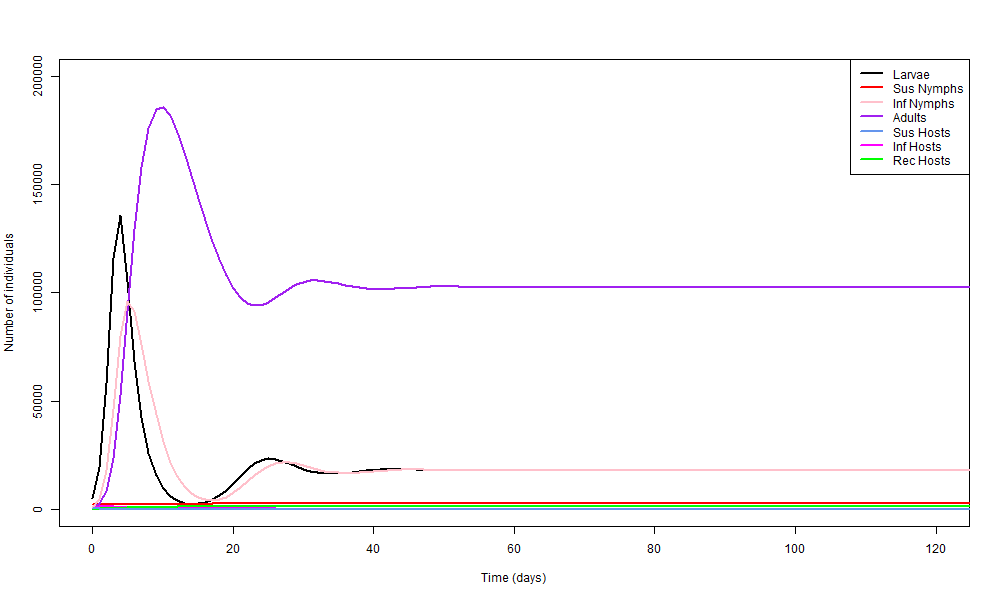
\includegraphics[scale = 0.4]{figures/base_large.png}
\end{subfigure}
\begin{subfigure}{\textwidth}
    \centering
    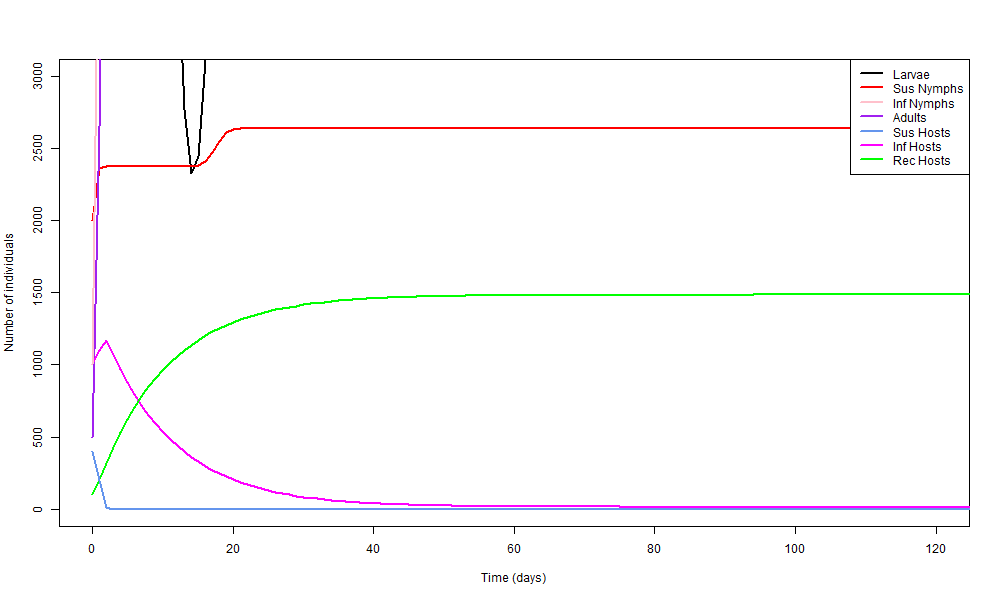
\includegraphics[scale = 0.4]{figures/base_small.png}
\end{subfigure}
\caption{Population dynamics of ticks and hosts}
\label{fig:base_model}
\end{figure}

\subsection{Rodent Bait Intervention}
Our model showed two equilibrium outcomes: one where Lyme disease is eradicated in the tick population and one supporting endemic Lyme disease. Assuming a consistent birth rate, this varies primarily on the delta value ($\delta$), per the equilibrium analysis performed in \cite{tosato2021host}. However, it is essential to note that the tick population itself does not die out and will remain susceptible to Lyme disease should it be reintroduced into the system without proper acaricide use. Figure \ref{fig:eradicated}, shown on a smaller population scale for ease of interpretation, represents the case where Lyme disease is eradicated, and Figure \ref{fig:endemic} represents the case where an endemic equilibrium is reached. Both are shown on a 120 day time scale, since this is approximately the duration of one season, and assume that the host population is 80\% saturated with acaricide.

\begin{figure}[h]
    \centering
    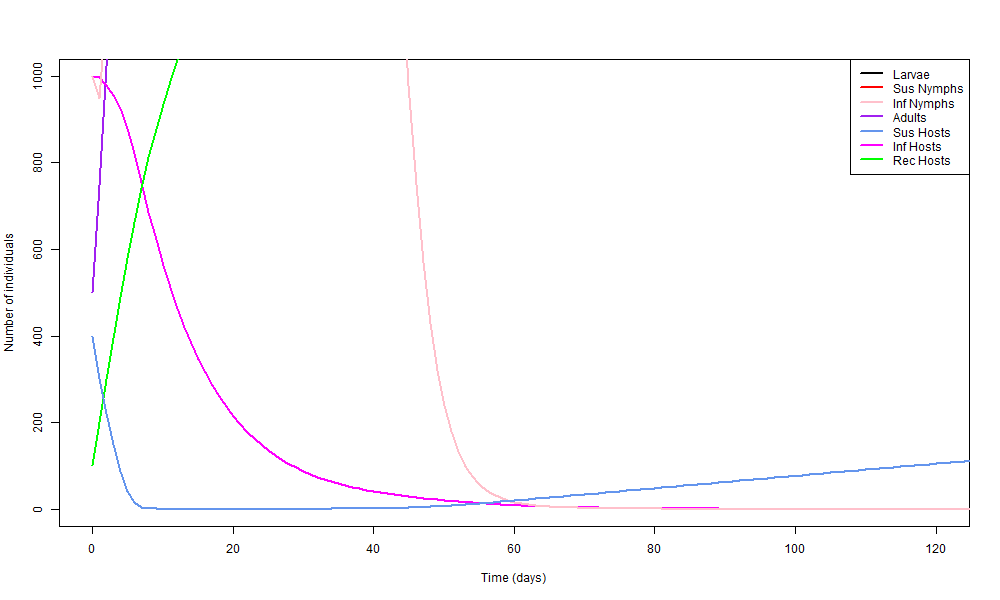
\includegraphics[scale = 0.4]{figures/intervention_eradicated.png}
    \caption{Lyme disease is eradicated when the value of $\delta$ is 0.1}
    \label{fig:eradicated}
\end{figure}

\begin{figure}[h!]
\begin{subfigure}{\textwidth}
    \centering
    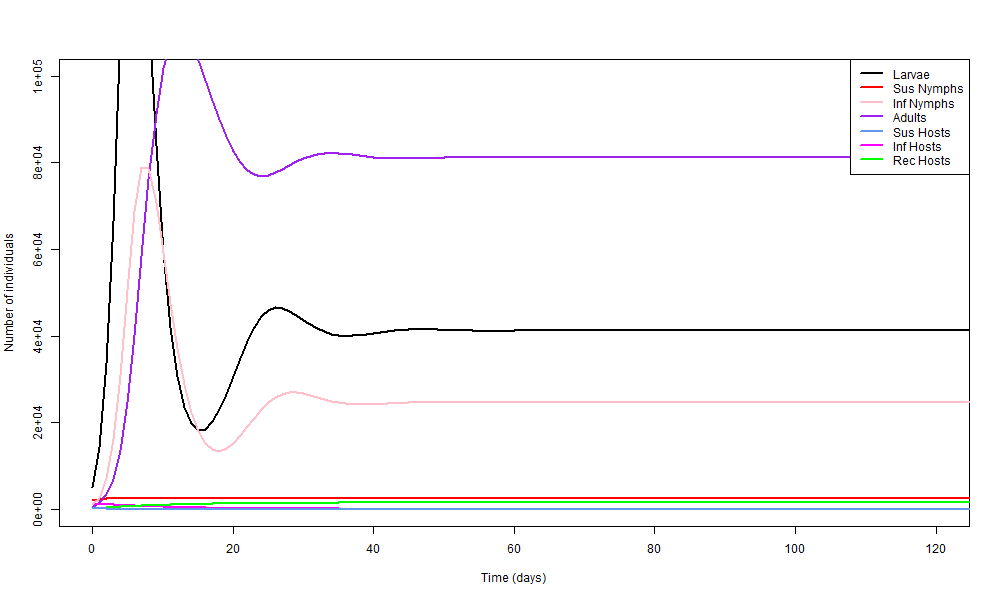
\includegraphics[scale = 0.28]{figures/intervention_40.png}
    \caption{Case when acaracide has a 40\% mortality rate}
\end{subfigure}
\begin{subfigure}{\textwidth}
    \centering
    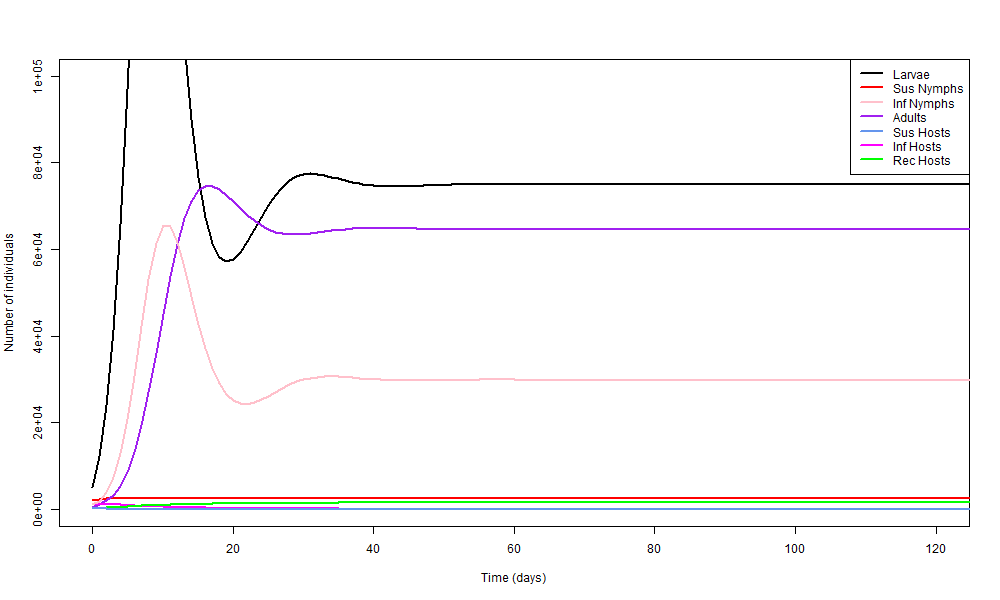
\includegraphics[scale = 0.28]{figures/intervention_60.png}
    \caption{Case when acaracide has a 60\% mortality rate}
\end{subfigure}
\begin{subfigure}{\textwidth}
    \centering
    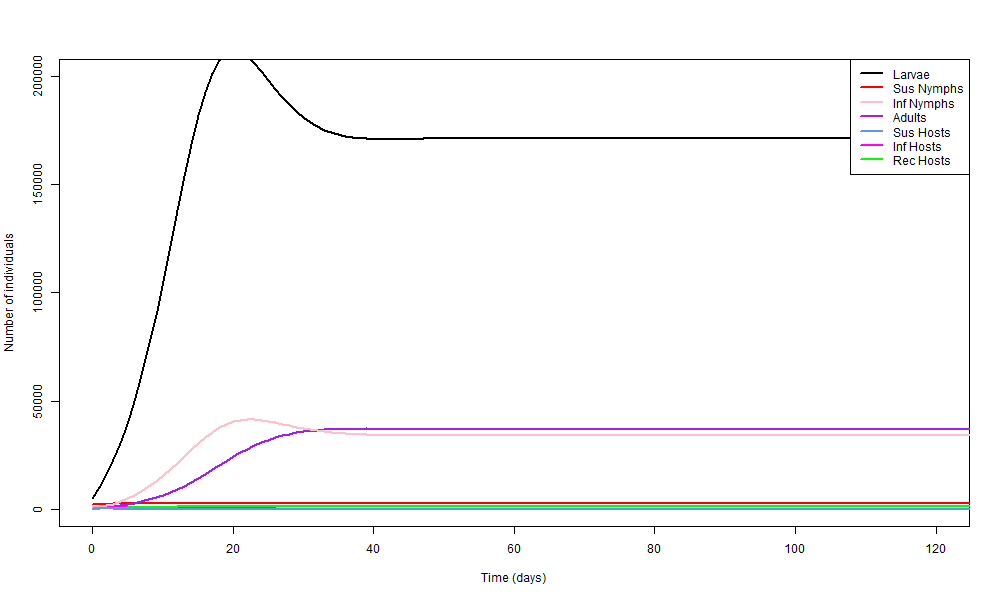
\includegraphics[scale = 0.28]{figures/intervention_endemic.png}
    \caption{Case when acaracide has an 80\% mortality rate}
\end{subfigure}
\caption{Lyme disease remains endemic when the value of $\delta$ is 0.7}
\label{fig:endemic}
\end{figure}

We see from Figure \ref{fig:eradicated} that the population of infected nymphs and hosts both reach 0 around 60 days in, meaning Lyme disease is no longer in circulation. 

Figure \ref{fig:endemic} shows three different cases where an endemic equilibrium is reached, based on possible variance in efficacy of the acaricide intervention. At the expected 80\% mortality rate, the population of infected nymphs and adult ticks rests at around 71 073 combined (34 132 infected nymphs, and 36 941 adults), which is around 50 000 less than in the case where no acaricides were used (120 369, with 17 816 infected nymphs and 102 553 adults). In conservative cases with 40\% and 60\% mortality rates, the populations of infected nymphs and adult ticks rest at around 105 817 and 94 541 respectively. Importantly, these are distinct improvements over the base model with no intervention.

\subsection{Uncertainty Analysis}
The uncertainty analysis for parameters pertaining to our acaricide intervention model for parameters resulting in the eradication of Lyme disease produced the following results in Figure \ref{fig:un_eradicated} over a 120-day period, corresponding to roughly four months. We also did a similar analysis shown in Figure \ref{fig:un_endemic} for the case where the acaricide intervention method results in an endemic equilibrium. The difference between these two scenarios is a matter of differing parameter values (most importantly, $\delta$).

\begin{figure}[h]
    \centering
    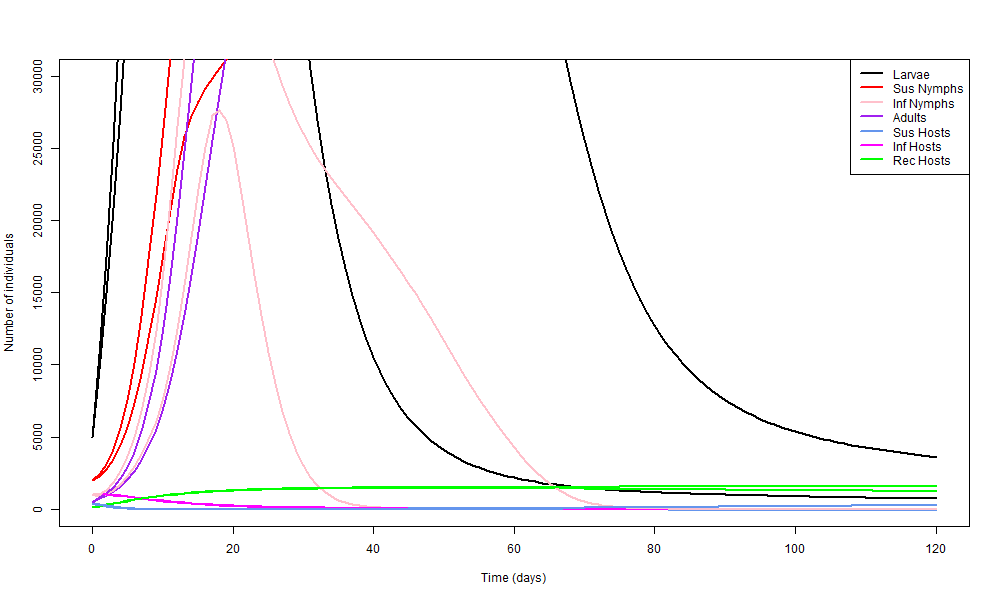
\includegraphics[scale = 0.4]{figures/uncertainty_eradicated.png}
    \caption{Uncertainty in population dynamics when $\delta$ is set such that Lyme disease will be eradicated and parameters are varied according to their assumed distributions}
    \label{fig:un_eradicated}
\end{figure}

\begin{figure}[h]
    \centering
    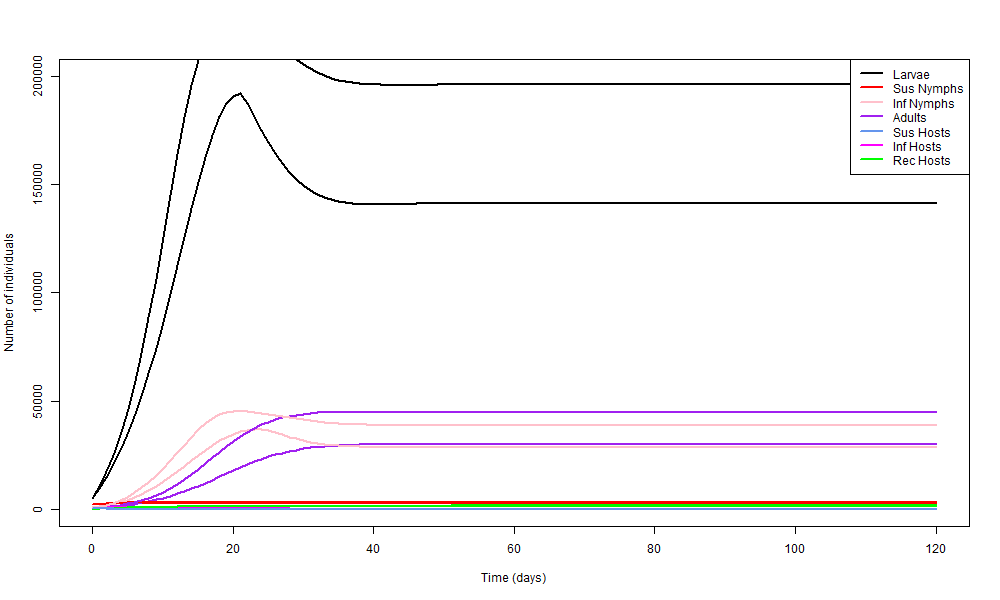
\includegraphics[scale = 0.4]{figures/uncertainty_endemic.png}
    \caption{Uncertainty in population dynamics when $\delta$ is set such that Lyme disease will remain endemic and parameters are varied according to their assumed distributions}
    \label{fig:un_endemic}
\end{figure}

The maximum and minimum values for all 1000 parameter sets were displayed for each compartment. From this, assuming the parameter distributions were chosen reasonably, we can conclude that with a setting mirroring ours, most real-world tick populations will lie within the ranges shown in our two graphs. Given that the variance of each parameter was quite low and that this still resulted in quite a wide range in some cases, it can be said that the parameters are relatively sensitive to change. Note that these values may vary drastically depending on the distribution method of the acaricide solution, along with factors such as temperature, season, and species population and diversity.

\section{Discussion}

\subsection{Model Implications}

In this project, we evaluated the effect of acaricide use in a rodent population on the spread of Lyme disease to ticks. We found that if a high proportion of rodents receive the acaricide treatment, the tick populations will suffer, thus reducing the propagation of Lyme disease to humans. These results are similar to the findings of \citet{tosato2021host}. The model did have a high level of sensitivity to parameter changes, making it less reliable than would be needed for actual policy implementation, however the basis that acaricides could prove effective for reducing Lyme disease is significant.


\subsection{Effect on Policy Decisions}

Interventions around Lyme disease can be introduced at various levels, such as host-level, tick-level and human-level. For example, current public health recommendations are to take physical precautions when entering areas with ticks, such as wearing bug repellent and light-coloured clothes to spot ticks \citep{govcan}. Most commonly, public health decisions around Lyme disease are made at a human level, such as physical prevention, vaccination, and immediate antibiotics. However, it is essential to consider host or tick-level interventions as effective public health measures. Lyme disease is a vector-borne disease where prevalence depends on host and tick interactions. %\sophie{i think the next few sentences need to be fixed for flow and stuff - ill do this later}
For example, studies show that the density of ticks and ticks with Borrelia are correlated with deer populations in that area, thus it can be inferred that Lyme disease proportion is also correlated. In fact, \citet{kilpatrick2014relationship}found an eighty percent reduction of resident-reported Lyme disease cases when the density of deer was reduced.  

Rodents are also a critical host when controlling tick abundance and, consequently, Lyme disease, as most ticks get infected with Borrelia when feeding on these rodents during their larval and nymph stages (see Figure \ref{fig:lifecycle}) \citep{radolf2012ticks}. The model used in this paper demonstrates that using acaricides on rodents via bait boxes can reduce the abundance of larvae and nymphs in a specific location. Public health and environmental health are connected through a One Health lens, and interventions introduced at an ecological level can influence the prevalence of vector-borne diseases. When fewer ticks are present, humans have a lower chance of interacting with them and consequently becoming infected with Lyme disease. 

If we do not consider early intervention, then suspected cases can cause a larger financial burden on the healthcare system as treatment, especially late treatment, is often less cost-effective than prevention interventions. For example, once an individual is suspected of being bitten by an infected tick or shows signs of early Lyme disease, they are usually treated with oral antibiotics, such as doxycycline and amoxicillin, for the course of 14 to 21 days to clear the bacteria \citep{borrelia_shapiro}. A later stage of the disease means that the medication period with this antibiotic will be longer and may be administered intravenously for complete recovery from the disease. Hence, it is important to consider environmental measures as a potential health policy to reduce Lyme disease by reducing infected tick abundance.

When exploring public health policies, it is important to consider the impacts of the interventions on social determinants of health, health economics and the healthcare system. Based on Table 3, topical acaricides are also better compared to other similar interventions, such as deer fencing and general acaricide, as preventive measures of interest in terms of all aspects.  In this study, the introduction of acaricides as an intervention for Lyme disease is effective, sustainable and can be cost-effective compared to other interventions. The bait boxes do not require frequent maintenance, with bait replenishment only needed approximately once a month \ref{tab:my-table}. Furthermore, the bait boxes will affect populations of Lyme disease hosts other than rodents, which means they still have the potential to be effective even if the ticks adapt to host preference. Bait boxes are not damaging to the environment in which they reside and can be placed sparsely or densely depending on host population density in an area. In summary, this intervention could allow for a potentially low-risk method to reduce Lyme disease in an area and can be easily controlled.
 



% Please add the following required packages to your document preamble:
% \usepackage{graphicx}
% \usepackage[table,xcdraw]{xcolor}
% If you use beamer only pass "xcolor=table" option, i.e. \documentclass[xcolor=table]{beamer}
\begin{table}[h]
\caption{Comparison of topical acaricides on rodents to other interventions in terms of range, social determinants of health, cost-effectiveness and environmental impact. }
\label{tab:my-table}
\resizebox{\textwidth}{!}{%
\begin{tabular}{
>{\columncolor[HTML]{C0C0C0}}l l}
\hline
\textbf{Interventions}                                & \cellcolor[HTML]{C0C0C0}\textbf{Topical acaricides}      \\ \hline
\textbf{Target   host/}                               & Rodents                                                  \\
\textbf{Impact on   tick abundance (population size)} & Yes   (Decrease)                                         \\
\textbf{Spatial   range of protection}                & Habitat with   rodents                                   \\
\textbf{Temporal   range of protection}               & 1 year                                                   \\
\textbf{The lag   time between use and protection}    & 1 year                                                   \\
\textbf{Social   determinants of health}              & No, as only   rodent species are impacted.               \\
\textbf{Cost-effectiveness}                           & Yes, only requires   a simple bait box and intervention. \\
\textbf{Environmental   impact} & Yes, as the   intervention only impacts ticks on the rodent. \\ \hline
\end{tabular}%
}
\end{table}
% Please add the following required packages to your document preamble:
% \usepackage{graphicx}
% \usepackage[table,xcdraw]{xcolor}
% If you use beamer only pass "xcolor=table" option, i.e. \documentclass[xcolor=table]{beamer}
\begin{table}[h]
\resizebox{\textwidth}{!}{%
\begin{tabular}{l}
\hline
\rowcolor[HTML]{C0C0C0} 
\textbf{Deer   fencing}                            \\ \hline
Deer                                               \\
Yes   (Decrease)                                   \\
Fenced area                                        \\
permanent (if   the fence is maintained)           \\
1 to 2 years                                       \\
No, as only   large mammals are impacted.          \\
No, requires   regular maintenance of the fence, as any breach will render intervention   inactive. \\
Yes, as the   intervention only acts as a barrier. \\ \hline
\end{tabular}%
}
\end{table}
% Please add the following required packages to your document preamble:
% \usepackage{graphicx}
% \usepackage[table,xcdraw]{xcolor}
% If you use beamer only pass "xcolor=table" option, i.e. \documentclass[xcolor=table]{beamer}
\begin{table}[h]
\resizebox{\textwidth}{!}{%
\begin{tabular}{l}
\hline
\rowcolor[HTML]{C0C0C0} 
\textbf{General   acaricide}    \\ \hline
Host-seeking ticks              \\
Yes (Decrease)                  \\
Treatment area                  \\
1 to 2 months                   \\
1 day                           \\
Yes, as the acaricides, once sprayed, can impact human health through accidental breathing of toxic   gas. \\
Yes, as the benefits of the acaricide outweigh the intervention cost                                       \\
Not environmentally sustainable \\ \hline
\end{tabular}%
}
\end{table}


\newpage
\section{Conclusion and Future Work}

In conclusion, topical acaricide on rodents is the best policy option against Lyme disease prevalence as it directly reduces tick abundance in a population. This preventative intervention is cost-effective, has low environmental impact and does not greatly impact social determinants of health in local populations. This is further reinforced when this intervention is compared to other similar interventions (deer fencing and general acaricides) and reactive interventions (treatment).

Future work considering acaricides as an intervention to prevent the spread of Lyme disease may consider furthering the model to include deer population migration, seasonality of tick and host populations, and even a spatial approach to investigate the interactions of hosts and bait boxes. 

\subsection{Further material}

To investigate the dynamics of the model used in this project, we created a Shiny app in R. This app allows users to modify the parameters and observe the behaviour of the population dynamics. Most significant is the ability to change the proportion of rodents treated with acaricide, in which case the dynamics of host and tick populations are important to policy makers. Find the app \href{https://stelmacs.shinyapps.io/Lyme_disease/}{here}.

\section{Acknowledgements}

We thank the director of the AARMS-EIDM Summer School, Dr. Amy Hurford, and the invited lecturers for sharing their knowledge and providing the opportunity to develop this project.

\newpage
\bibliographystyle{chicago} %idk what style we want to do
\bibliography{bib}
\end{document}
